\documentclass[10pt]{article}
\usepackage{natbib}
\usepackage{mathtools}
\usepackage{graphicx}
\usepackage{lscape}
\begin{document}
\begin{titlepage}
\title{The experimental determination of the relationship between stress, strain, acoustic velocity and density in greenwood \textit{Pinus radiata}}
\author{Nicholas Davies, Clemens Altaner and Luis Apiolaza}
\maketitle
\emph{New Zealand School of Forestry, University of Canterbury}
\begin{abstract}
This paper presents a number of important constants needed for the use of
 mathematical modelling of greenwood \textit{Pinus radiata}. The constants include all three necessary Youngs and shear
 moduli along with the six Poisson ratios needed for describing orthotropic materials in the elastic domain.
 Further yield surfaces and ultimate tensile strength are investigated. The accuracy of the various measurements are discussed in detail.
\end{abstract}

\thispagestyle{empty}
\end{titlepage}
\pagenumbering{arabic}
\setcounter{page}{1}

\section{Introduction}
While density and acoustic tests are common practice for obtaining dynamic modulus (which can in turn be used to estimate
the static modulus \citep{barker_properties_1998,lindstrom_stiffness_2004}) in both timber research and industry, little
information about the underlying structure of wood is obtained from these tests. Wood is often dried to 6-12\% moisture
content before conducting any experimental work, which has been observed to alter the mechanical properties
\citep{skaar_springer_1988,ozyhar_moisture-dependent_2013}. Investigating dry wood gives a poor representation of the
living organism, leaving scientists interested in the growth of trees somewhat in the dark when considering the way trees
react to mechanical phenomenan. Unfortunately there is a lack of information on both green (the state of wood when it is inside
a living tree) and core wood (wood produced by a young cambium).

Wind loading can cause mechanical failure which can decrease the value of processed timber due to defects, the associated financial
loss has led to a substantial amount of research on predicting wind throw and wind damage risk for commercial species
\citep{gardiner_review_2008}. However, these models do not investigate the structural failure within the tree,
they only attempt to identify how likely failure is to occur in a particular environment. In areas with less pronounced
prevailing wind directions there may be an effect on the stiffness of the trees in order to compensate for the multi-directional
loadings \citep{apiolaza_characterization_2011,kern_mechanical_2005}, this reduction in stiffness can result in a timber product
of lower value.

One way of investigating mechanical phenomenon present in tree stems is the use of mathematical models, using the
Finite Element Method (FEM). However because of the size of the tree, modelling an entire tree from the molecular
level is infeasible, so homogenization is used. In order to use these methods experimental data is required to parametrize them.
Full sets of constants even for dry timber are hard to find and to the best of our knowledge there are no full sets available
for green or core wood radiata. Proportional limit and ultimate failure surfaces for all directions in green and core wood
have also not been reported previously. Lack of available data is an issue for a number of current problems in plant biophysics.

The purpose of this paper is to present a number of necessary material constants
for describing green core and outer wood as an orthotropic material.
A set of static moduli and Poisson ratios for green core and outer wood in the radial, tangential
and longitudinal (to the grain) directions. The small study was completed with \textit{Pinus radiata}
selected from plantations in Canterbury, New Zealand.

\section{Experimental Method}
\subsection{Sample Selection and Preparation}
Green radiata pine (\textit{Pinus radiata}) samples were sourced from a sawmill
in Canterbury, New Zealand. Four boards were chosen from approximately
30 boards to represent extremes of outerwood and corewood based on green density
and dynamic modulus (Table \ref{table:mill samples table}). Green dynamic
modulus was calculated from acoustic velocity measurements and green mass \citep{Chauhan_methods_2013}.

The samples were docked into approximately 500 mm lengths and stored in sealed
bags with excess water at 5\(^\circ C\)  subsequently 6 defect-free, straight
grained test specimens of the required shape and orientation were machined from each of
the four boards and stored in sealed bags with excess water until testing.
Prior to mechanical testing each specimen was weighed and it's volume measured
by water displacement.

\subsection{Testing}
The specimens were placed into a Universal Testing Machine (UTM)(Instron 5566)
set-up for the appropriate test. Displacement was tracked on the two faces
perpendicular to the axis of loading with two digital cameras fitted with 60 mm
micro lenses. Timelapse photography was used taking images
every 3 seconds during the test, controlled via gphoto2 \citep{contributors_gphoto2_2002}.

For compression testing, samples approximately 15 x 15 x 30 mm were used with
their grain oriented in longitudinal, radial or tangential direction.
The UTM fitted with a x KN load cell having an accuracy of 0.1 N was run at a
constant velocity of 1.5 mm per min for 300 seconds applying compression to the
top of the sample.

Tension testing used bone shaped samples with dimensions approximately 50 x 25 x
6.5 mm with the breakage plane having an area of approximately 6.5 x 6.5 mm.
With the exception of the longitudinal direction, where a straight stick test was used.

For the shear plane L shaped samples with a shear plane approximately 15 x 15 mm
was used.

Once the specimens had been mechanically tested they were oven dried at 104\(^\circ C\) until a representative sample was no
longer losing weight 48 hours apart. Each sample was weighted and volume measured using the displacement method.
From one specimen of each sample and test (ie 12 in total) a small strip approximately 1 x 5 x 10 mm was taken for
x-ray diffraction testing. The micro-fibril angle and standard deviation of the micro-fibrils were obtained using the
methods described in \citet{cave_measuring_1998} and \citet{cave_interpretation_1998}.

The time and load applied was extracted from the UTM data for use with the photo collections to create stress strain curves.
This was implemented using Digital Image Correlation and Tracking with Matlab scripts
\citep{chris_eberl_robert_thompson_daniel_gianola_digital_2006} to track identifiable points within the photos throughout
each series to obtain strain  versus photo number curves. The time of each photo was obtained from the EXIF data attached
to the photo obtained from the Python Imaging Library \citep{lundh_python_1995} and used to match the corresponding
load applied by the UTM along with the dimension measurements which are used to calculate the stress strain curves.

During the process of extracting strain information from the images, a visual inspection of the data was undertaken.
This involved using displacement versus image number, displacement vs neighbour's displacement and area of interest selection
(available from \citet{chris_eberl_robert_thompson_daniel_gianola_digital_2006}) to determine the points which have been
tracked correctly within the photo series. One-Dimensional average strains are taken in both the vertical and horizontal direction.

Because the UTM runs at a set velocity it is possible to estimate the strain on the sample, although this tends to slightly
overestimate the strain. Initially there is a period of motion before the compression plate comes into contact and re orientates
the sample, (although this is minimal) providing a good estimation to select the accuracy tracked points.
The horizontal direction within the photographs is used to track the displacement perpendicular to the applied load.
Here the assumption is made that points tracked accuracy in the vertical
direction are tracked reliably in the horizontal direction.

\subsection{Calculation of the Elastic Modulus}
\label{sec:calc_E}
For each test of each specimen a visual inspection of the stress strain curves is undertaken, the initial reorientation of the sample,
resulting in a curve before the linear elastic region is discarded, and the linear portion of the stress strain curve identified
by overlaying a linear model \(y=mx\) to the data being considered. Once there was as little deviation between the data and model
as possible, this was considered the elastic region with the Elastic modulus \(E\) being the gradient \(m\) of the model.
The end point of the fitted model is considered the limit of proportionality, and it is assumed this is equal to the yield point.
This may provide a slightly lower yield point estimate than some other techniques for determining the yield point, such as taking the
 intersection  between this line and the line tangent to the peak of the plastic curve.

\subsection{Calculation of the Poisson Ratios}

Poisson ratios defined as \(v = -d\epsilon_x /d\epsilon_y \)  \citep{bodig_jozsef_jayne_mechanics_1982} (where \(\epsilon\)
is strain, \(x\) is transverse direction and \(y\) is axial direction) from the method in section \ref{sec:calc_E} the slope
of the elastic region of the stress strain curve is known for both the \(x\) and \(y\) directions. In \(y\) this is the Young's
Modulus, defined as \(E_y = \sigma_y / \epsilon_y\) (where \(\sigma\) is stress)  \citep{bodig_jozsef_jayne_mechanics_1982} and
in the \(x\) direction \(S_x = \sigma_y / \epsilon_x\) (i.e. the force per unit area applied in the \(y\) direction results in a
displacement in the \(y\) and a different displacement in the \(x\) direction related by the Poisson ratio).
Therefore \(S_x = \sigma_y / \epsilon_x \) and \(E_y = \sigma_y / \epsilon_y\) so \(-\epsilon_x / \epsilon_y = E_y/S_x\)
giving \(v_{yx} = -E_y/S_x\)

\subsection{Determining Elastic Moduli and Poisson ratios for use with the orthotropic assumption}
\label{sec:orthotropic_assumption}
Orthotropic materials have symmetry giving rise to the following equalities \citep{salencon_handbook_2001}:

\begin{equation}\label{eqn:equalities}
\frac{v_{yx}}{E_y}=\frac{v_{xy}}{E_x},\hspace{0.5cm} \frac{v_{zx}}{E_z}=\frac{v_{xz}}{E_x},\hspace{0.5cm} \frac{v_{yz}}{E_y}=\frac{v_{zy}}{E_z}
\end{equation}

However from the experiments the equalities presented in equation \ref{eqn:equalities} do not hold. This is probably due
to a number of reasons, such as the errors inherent in the method of measurements. In order to ensure these equalities hold (which is necessary for the assumption of wood being an
optimization is used to find the values which deviate least from all of the
experimental values while still satisfying the equality constraints above. Due to the larger absolute values of some constants (for example \(E_l\))
the deviation is considered as normalized against the 95\% confidence intervals of the mean values in order to give every
variable an even weighting for its accuracy. The optimization uses the above constraints and the following objective function:
\begin{equation}\label{eqn:min}
min\sum \frac{|\delta_i - \gamma_i|}{ \theta_i} \hspace{0.5cm} i = E_r, E_t, E_l, v_{rt}, v_{tr}, v_{tl}, v_{lt}, v_{lr}, v_{rl}
\end{equation}
Where \(\delta_i\) is the experimental value of \(i\), \(\gamma_i\) is the new value and \(\theta_i\) is the 95\% confidence
interval of \(\delta_i\). This optimization was implemented in a least squares sense using the  python algorithm
scipy.optimize.fmin\_slsqp \citep{jones_scipy:_2001}. It should be noted that setting the 95\% confidence intervals as bounds
worked for all but one case. The Stiff Outerwood sample when tested under tension fails to converge, due to the inequality
constraints being incompatible with any combination within the bounds. This is redeemed by increasing the bound to the 99.9\%
confidence intervals. An average of  Elastic moduli obtained from both compression and tension tests was also undertaken.
For the \(r\) and \(t\) directions the values from the non axial plane for each tension and compression were averaged,
whereas for the \(l\) direction all measurements were averaged. The Poisson ratios from compression tests were used.
The reasons for using these particular values are discussed in section \ref{sec:dis_error}.

\subsection{Proportional limit (Yield point) Criteria and ultimate failure}
\label{sec:TW}
The failure criterion presented by \citet{tsai_general_1971} provides a general theory of strength for anisotropic materials,
other papers have since used this failure criterion and it has been suggested as an appropriate failure criterion for wood and
wood products \citep{mackenzie-helnwein_rate-independent_2005,mackenzie-helnwein_analysis_2005}.
Due to the use and acceptance of the theory in other research along with its treatment of experimental results allowing for pure
tension and compression to be regarded separately make it a good choice for investigation into the properties of green wood.
The separate treatment of pure tension and compression is needed as wood has been reported to behave substantially differently
under the two regimes \citep{ozyhar_moisture-dependent_2013,bodig_jozsef_jayne_mechanics_1982}. Shear loading is extremely
difficult to test within wood due to the material structure being very week in planes perpendicular to the longitudinal axis
(i.e. separation between cells requires much less force than breakdown of the cells themselves). The problem of separation is
evident in shear tests where the samples are likely to split under the rotational loading (although this loading is assumed to
be negligible, it is often significant \citep{bodig_jozsef_jayne_mechanics_1982}) between the cells rather than fracture through
the desired plane. In the future this could be overcome by using different equipment and more sophisticated shear tests such as
those presented in \citep{bs_methods_1957} or  \citet{kollmann_f._cote_principles_1968}. It has also been suggested that shear
properties are best derived from torsion or various bending tests \citep{moden_micromechanics_2008}.

The full power of \citet{tsai_general_1971} failure criterion was not used in this paper. The off axis interaction terms are ignored.
The implementation of Tsai and Wu's failure criterion is described in equation \ref{equ:TW}
\begin{equation}\label{equ:TW}
\boldsymbol{\sigma}^T\boldsymbol{q} + \boldsymbol{\sigma}^T\boldsymbol{P\sigma} -1 = 0
\end{equation}
Where:
\begin{equation}\label{equ:stress_vec}
\boldsymbol{\sigma}=\begin{bmatrix}
	\sigma_{r}\\
	\sigma_{t}\\
	\sigma_{l}\\
	\sigma_{tl}\\
	\sigma_{lr}\\
	\sigma_{rt}
	\end{bmatrix}
\end{equation}
\hspace{0.2cm}
\begin{equation}\label{equ:q_vec}
\boldsymbol{q}=\begin{bmatrix}
	F_{rr}\\
	F_{tt}\\
	F_{ll}\\
	0\\
	0\\
	0
	\end{bmatrix}
\end{equation}

\begin{equation}\label{equ:P_mat}
\boldsymbol{P}=\begin{bmatrix}
	F_{rrrr}&F_{rrtt}&F_{rrll}&0&0&0\\
	F_{rrtt}&F_{tttt}&F_{ttll}&0&0&0\\
	F_{rrll}&F_{ttll}&F_{llll}&0&0&0\\
	0&0&0&F_{tltl}&0&0\\
	0&0&0&0&F_{lrlr}&0\\
	0&0&0&0&0&F_{rtrt}
	\end{bmatrix}
\end{equation}

with \(\boldsymbol{\sigma}\) as the stress vector, \(F_{ii}\), \(F_{ij}\), \(F_{iiii}\) and \(F_{ijij}\) described in
equations \ref{equ:F_vals1} to \ref{equ:F_vals4}:

\begin{equation}\label{equ:F_vals1}
F_{ii} = \frac{1}{f_{it}}-\frac{1}{f_{ic}} \hspace{0.5cm} i = r,t,l\hspace{0.2cm}\\
\end{equation}
\begin{equation}\label{equ:F_vals2}
F_{ij} = \frac{1}{f_{ijt}}-\frac{1}{f_{ijc}} \hspace{0.5cm} i,j = r,t,l \hspace{0.2cm} (i\neq j)\hspace{0.2cm}\\
\end{equation}
\begin{equation}\label{equ:F_vals3}
F_{iiii} = \frac{1}{f_{it}f_{ic}} \hspace{0.5cm} i = r,t,l\hspace{0.2cm}\\
\end{equation}
\begin{equation}\label{equ:F_vals4}
F_{ijij} = \frac{1}{f_{ij}^2} \hspace{0.5cm} i,j = r,t,l \hspace{0.2cm} (i\neq j)
\end{equation}


Where \(f_{it}\) and \(f_{ic}\) are the tensile and compressive strengths in the \(i\) direction with \(f_{ij}\) the shear strengths.
In a simplified case  \(F_{iijj}\) is ignored giving the following \(\boldsymbol{P}\) matrix with no interaction terms:

\begin{equation}\label{equ:P_mat_k0}
\boldsymbol{P}=\begin{bmatrix}
	F_{rrrr}&0&0&0&0&0\\
	0&F_{tttt}&0&0&0&0\\
	0&0&F_{llll}&0&0&0\\
	0&0&0&F_{tltl}&0&0\\
	0&0&0&0&F_{lrlr}&0\\
	0&0&0&0&0&F_{rtrt}
	\end{bmatrix}
\end{equation}

The system of equations is solved using optimization techniques. As only two of the six stresses are of interest at any one time
(due to visualisation requirements), one is set as the independent variable and a linear space set-up to provide each point that
will be evaluated (\(n=1000\)), the other four stress directions which are not of interest are set to 0, and the dependent variable
is calculated by maximising the distance \(\sqrt{\sigma_{independent}^2+\sigma_{dependent}^2}\) subject to equation \ref{equ:TW},
completed using the scipy.optimize.fmin\_ slsqp algorithm \citep{jones_scipy:_2001}.
The proportional limit criterion (assumed to be the same as the yield criterion) is reported in all directions, however the
ultimate failure criterion is only reported for the tensile tests. In the tensile direction ultimate failure is characterised
by very quick drop in stress to near zero, this happens when the sample breaks into two parts. In the compressive direction ultimate
failure is harder to define, if it is considered as the start of sample densification, the experimental results in this study are unable
to provide the required information. The tests were limited to a maximum strain of 0.25. Other studies in dry wood have shown densification
starts at strains greater than 0.5 \citep{gibson_l._ashby_cellular_1997}. When considering the tree as a living structure it is hard to
conserve of a case in nature where densification would occur without ultimate tensile failure occurring on the opposite side of the stem.


\section{Results and Discussion}

A number of descriptive properties of the samples are presented in Table \ref{table:init properties}.
As is widely reported the outer wood boards were of higher dry density and lower
MFA (and in turn faster acoustic velocity) resulting in higher axial dynamic
modulus. It is important to note that the variation between the extremes is
larger in corewood than between outerwood samples with the stiff corewood sample
being of similar properties as the outerwood.

% The optimised elastic moduli and Poisson ratios are given in Table
% \ref{table:optermised vals}, with the Poisson ratios obtained from the
% compression tests, as displacment measures in tensions were at the detection
% limit.

The Elastic moduli and Poisson ratios here were obtained through the
optimization and averaging.
Table \ref{table:optermised vals average} uses Poisson ratios from the compressive tests, the Elastic moduli from non-longitudinal faces
where possible and all four faces for the axial direction. Tension and compression values are averaged and optimised.

Figure \ref{fig:yeild, k0} shows the failure planes calculated as described
above with no interaction terms. The behaviour of the two core wood samples are
of interest, while the outer wood samples are stronger in longitudinal tension than compression, the core wood samples are much more centred on the zero axis.

Experimentally obtained values are reported in Table \ref{table:yield points}. Measurements of the same directional force
(eg, \(lr_t\) and \(lt_t\) could be averaged, as they are both measurements of the same  phenomenon.

Table \ref{table:ultimate strength} presents multiple measurements of the same tests,
reported here as \(lr\) and \(lt\), \(rt\) and \(rl\), \(tr\) and \(tl\). These can be averaged to calculate the three
ultimate strengths, but are reported separately for completeness.

The proportional limit surfaces show the propensity for wood to be stronger in the axial tensile direction than any other when considering
the high density (outerwood) samples. An interesting phenomenon occurs with decreasing density, the samples become more centred or even
favour compression in the longitudinal direction. Both corewood samples indicate
the compressive strength is much more important than it is in the outerwood samples
(which follow the more traditional idea of higher strength in tension).
Some examples that might have an impact on this are the low second moment of area from the thin
stem meaning the tree must withstand much more movement from wind, resulting in more compression wood like cells being produced
 at young ages. Animals stepping on stems causing compressive destruction may have an effect.
 The trend may also be a by product of a non mechanical pressure. It is possible that because these samples were taken from
 fully growth trees, (typically 25-30 years old) that over time the material structure has been degraded by growth stresses,
 or other time/growth dependent phenomenon resulting in a reduction in tensile strength, which is not present if the wood is tested
 from a young tree.

%All samples show that under radial or tangential loading that compressive
%stress is favoured. This may be due to the different failure mechanisms in
% tension and compression, with tension causing peeling between the cells, while compression must act on the cells themselves. If there has been no evolutionary pressure causing the cells to reinforce the connection to resist tension it may
%result in a significantly lower proportional limit than in compression where
% the geometry of the cellular structure gives it more strength.

% The Tsai and Wu criterion has been used in a number of papers as discussed in section \ref{sec:TW} however it has been suggested that
% the criterion is insufficient \citep{p_multi-surface_2003,mackenzie-helnwein_rate-independent_2005}. Because we have assumed linear
% elastic deformation, with the yield point defined as the end of the linear section of the stress strain curve, no non-linear elastic
% effects have been considered. These authors suggested that the non-linearity which is usually considered to be non-linear elastic is due
% to an inelastic portion of the the total strain, so these findings should have little effect on these results.

The Elastic and Shear moduli are low although similar to published values for dry wood, as are the Poisson ratios, as can be seen
in Tables \ref{table:lit_comp} and \ref{table:lit_comp_long}. The lower values presented here are not unexpected due to the samples
being in green condition and from \textit{Pinus radiata}. In order to accurately quantify the differences between green and dry wood
values more accurate testing procedures along with a higher number of samples are needed.

Corewood needs further investigation as this study provides some interesting results, particularly the failure planes in the
longitudinal direction. With the corewood samples providing a higher ratio of compressive to tensile strength than outerwood samples.
Investigation is needed to determine if this is a property of core wood produced by seedlings and young trees, or if it forms
differently and is modified over time while the tree grows. Again to accurately quantify the difference between dry and green wood
properties a larger number of more accurate tests are needed.

It should be kept in mind that only four boards were tested during this experiment and those boards were selected as extreme cases of
green density and acoustic velocity. The selection criteria and low sample number result in the selected samples not being representative
of the species in general. In order to gain an understanding of the 'average' stem further testing is needed.

% It can be noted from Table \ref{table:mill samples table} that for the given green densities and acoustic velocities obtain using the
% disk scanner if one were to calculate the dynamic modulus, which has been reported to have a strong correlation to static modulus in
% the axial direction \citep{lindstrom_stiffness_2004,lindstrom_methods_2002} at usually around a \(1:1\) linear relation the predicted
% values for the axial modulus become very high. The disk scanner has not been used for samples of this shape before and as a consequence
% may not have been providing accurate velocities as they differ substantially from those obtained from wood spec.  The use of green wood
% may also have had an effect. The ranking of the samples does however fit with the persevered ranking when the boards were selected at the
% mill, and the density values. Both the acoustic velocities, green and dry densities, in general, have higher values for higher strength
% and stiffness boards. Low density core-wood samples have a low strength and stiffness compared to the outer-wood samples.

% Because in many cases a number of constants could be obtained by different methods from one or more tests there is a need to select the
%  measurements which best resemble the real underlying physical characteristics. While all of the results are reported above for
%  completeness, the following is a discussion to consider which are the more accurate solutions.

% Measurements in the horizontal direction can be ignored when considering tensile tests, this is due to the resolution of the
% cameras not being high enough to resolve the contraction on the samples in the horizontal direction. The low tensile strength
% in the radial and tangential directions results in very low dimension changes before both the proportional limit and the rupture
% of the sample. Although in the longitudinal direction the samples have a much higher breaking strength the reliability of the
% measurements of contraction in the horizontal direction is also suspect. Generally tracking of the longitudinal face of the samples
% is more error prone than the other two faces, it is suspected this is because of the uniformity of the image over the samples in
%  this direction, whereas in the other two directions early and late wood give identifiable points within the images used by the
%  point tracking algorithm. In the vertical direction the samples are tracked more reliably due to the greater number of pixels and
%   the greater displacement of the sample due to its shape. In the future artificially adding a random speckle pattern should be
%   considered to increase the accuracy of point tracking.

% Extension data extracted from the UTM can be ignored for all tension tests as the jaws which hold the sample are self tightening
% using a mechanism which provides an increase in extension reading at the machine without it being transferred to the sample.
% On samples of this size the effect was significant.
%
% Compression tests are used for calculating all of the Poisson ratios. Absolute values of constants obtained from tracking on
% longitudinal faces appear to be low, however the Poisson ratios generally agree with the ratios gained from the other tests.
% Due to the implementation of the image tracking algorithm, if the algorithm does not detect the identifiable group of pixels
% in the new image it simply leaves the point with no displacement. It is suspected that the assumption that points tracked well
% in the vertical direction will also be tracked well in the horizontal direction holds true, along with its corollary, points
% which remain stationary due to poor tracking in the vertical direction will also remain stationary in the horizontal direction.
% The result of this is that although the absolute values for the displacement in both directions is highly suspect the ratio of
% observed displacement in the vertical and horizontal direction still provides a good estimate of the true value of the ratio
% because every time a displacement is observed in one direction, the associated displacement in the other direction is also observed.
% Because of the errors in the magnitude of the displacements when it can be avoided these values were not used. This not possible
% when calculating Poisson ratios, or the elastic modulus when force is applied in the longitudinal direction, as both cameras image
% a longitudinal face. For the radial and tangential directions of compression and tension the elastic modulus was calculated from
% the camera which had a view of the growth rings and hence provided more robust image tracking.

% The nature of shear tests means some of the force applied is dissipated through rotation of the sample block, the magnitude of
% this is expected to be significant due to the unexpectedly low values for the shear moduli. In some cases this rotational force
% results in breakage of the sample specimen via cell wall peeling in the plane perpendicular to the desired shear plane.
% Where the shear plane attempts to break the cells directly (ie shear plane perpendicular to the cell axis) bowing is observed
% around the bottom sample rest, this also dissipates energy further reducing the accuracy of the tests. It is worth noting that
% other testing methods for determining shear characteristics such as those presented in \citep{bs_methods_1957} and
% \citep{kollmann_f._cote_principles_1968} may provide more reliable solutions however these require more specialist equipment.
% The difficulty in obtaining accurate shear measurements has been reported on before
%  \citep{kollmann_f._cote_principles_1968, bodig_jozsef_jayne_mechanics_1982}. \citet{kollmann_f._cote_principles_1968}
%  reported shearing stress perpendicular to grain are 3-4 times higher than parallel to it.

%
% It can be seen from the data tables that generally the compressive tests result in higher elastic modulus values than
%  the tension tests. One explanation for this may be the documented dependence of the moduli on the dimensions of the
%  sample \citep{niklas_mechanical_1997}, with the tension tests being smaller than the compression tests this may lead
%  to lower outcomes. However what this does not explain is why the tension tests in the longitudinal direction of the
%  two outerwood samples (Stiff Outerwood and Non-Stiff Outerwood) are substantially larger than those in compression.
%  Another possible reason for this is that it is a genuine material property which is accentuated in outerwood indicating
%   it may be less well described by the assumption of an orthotropic material than core wood.

% When testing in pure compression or tension producing samples which are exactly in the desired direction is near
% impossible due to the variations in properties during the growth of the tree. While every effort was taken to minimise
%  the effect of this, in some cases, particularly in core wood with wide grain spacing it is not possible for the given
%   sample size, due to the radius of the rings. The Poisson ratios may be affected by the specimen not having all three
%   directions perfectly perpendicular. Some samples may be cut from boards with spiral grain but no samples with visible
%   spiral grain were used. It is thought that while this is an issue to note, it is unlikely to be substantially decrease
%   the accuracy of the measurements given the magnitude of other errors also discussed here.

% During compression testing it was observed that samples compressed in the tangential direction tend to bow in the same
% direction as the grain, this is much more evident in corewood where the curvature of the grain is larger.
% The bending may have some effect on the accuracy of the findings, but to what extent is unknown.

% It has been reported that the size of samples of wood when tested for elastic constants can have an effect on the
%  result \citep{niklas_mechanical_1997}. While size dependence is an important note to be aware of controlling for
%  this would require using samples which do not necessarily provide a good representation of a homogeneous piece of wood.
%  The sample sizes in this study most likely also suffer when compared to other tests utilising different sized samples.
%  It is important to use data collected from specimens which best represent the level of homogenisation required for the
%  particular end use. Given current personal computing resources, this size specimen provides a good resolution for finite
%  element models of an entire stem in the horizontal plane. The vertical direction shows much lower deviation of material
%  properties per unit length, so the sample dimension is less important, hence can be reduced in order to give clean samples
%  without defects.
%
% Experimental errors from changing dimensions within the UTM under loading are assumed to be negligible (with the exception
% of the mechanisms of the jaws used for tension tests). The load cells are reported to be accurate to 0.1N and hence are also
% negligible when compared to the major sources of error in these tests, the image tracking.

This paper did not consider interaction terms within the \textbf{P} matrix, \citet{tsai_general_1971} suggest the use of
experimentation to find the appropriate interaction terms for use within their strength criterion. Further research should
not only focus on increasing the size and accuracy of data sets of anisotropic constants but also include these interaction
terms to increase the accuracy of further calculation.

\pagebreak

\bibliography{exp_paper}{}
\bibliographystyle{apalike}

% \pagebreak
% \begin{figure}[!ht]
% \begin{center}
% \includegraphics[width=0.7\columnwidth]{figs/setup.jpg}
% \caption[Experimental layout]{\label{fig:setup} The layout of the instron and cameras for compression testing. The other setups are similar.
% }
% \end{center}
% \end{figure}
%
% \begin{figure}[!ht]
% \begin{center}
% 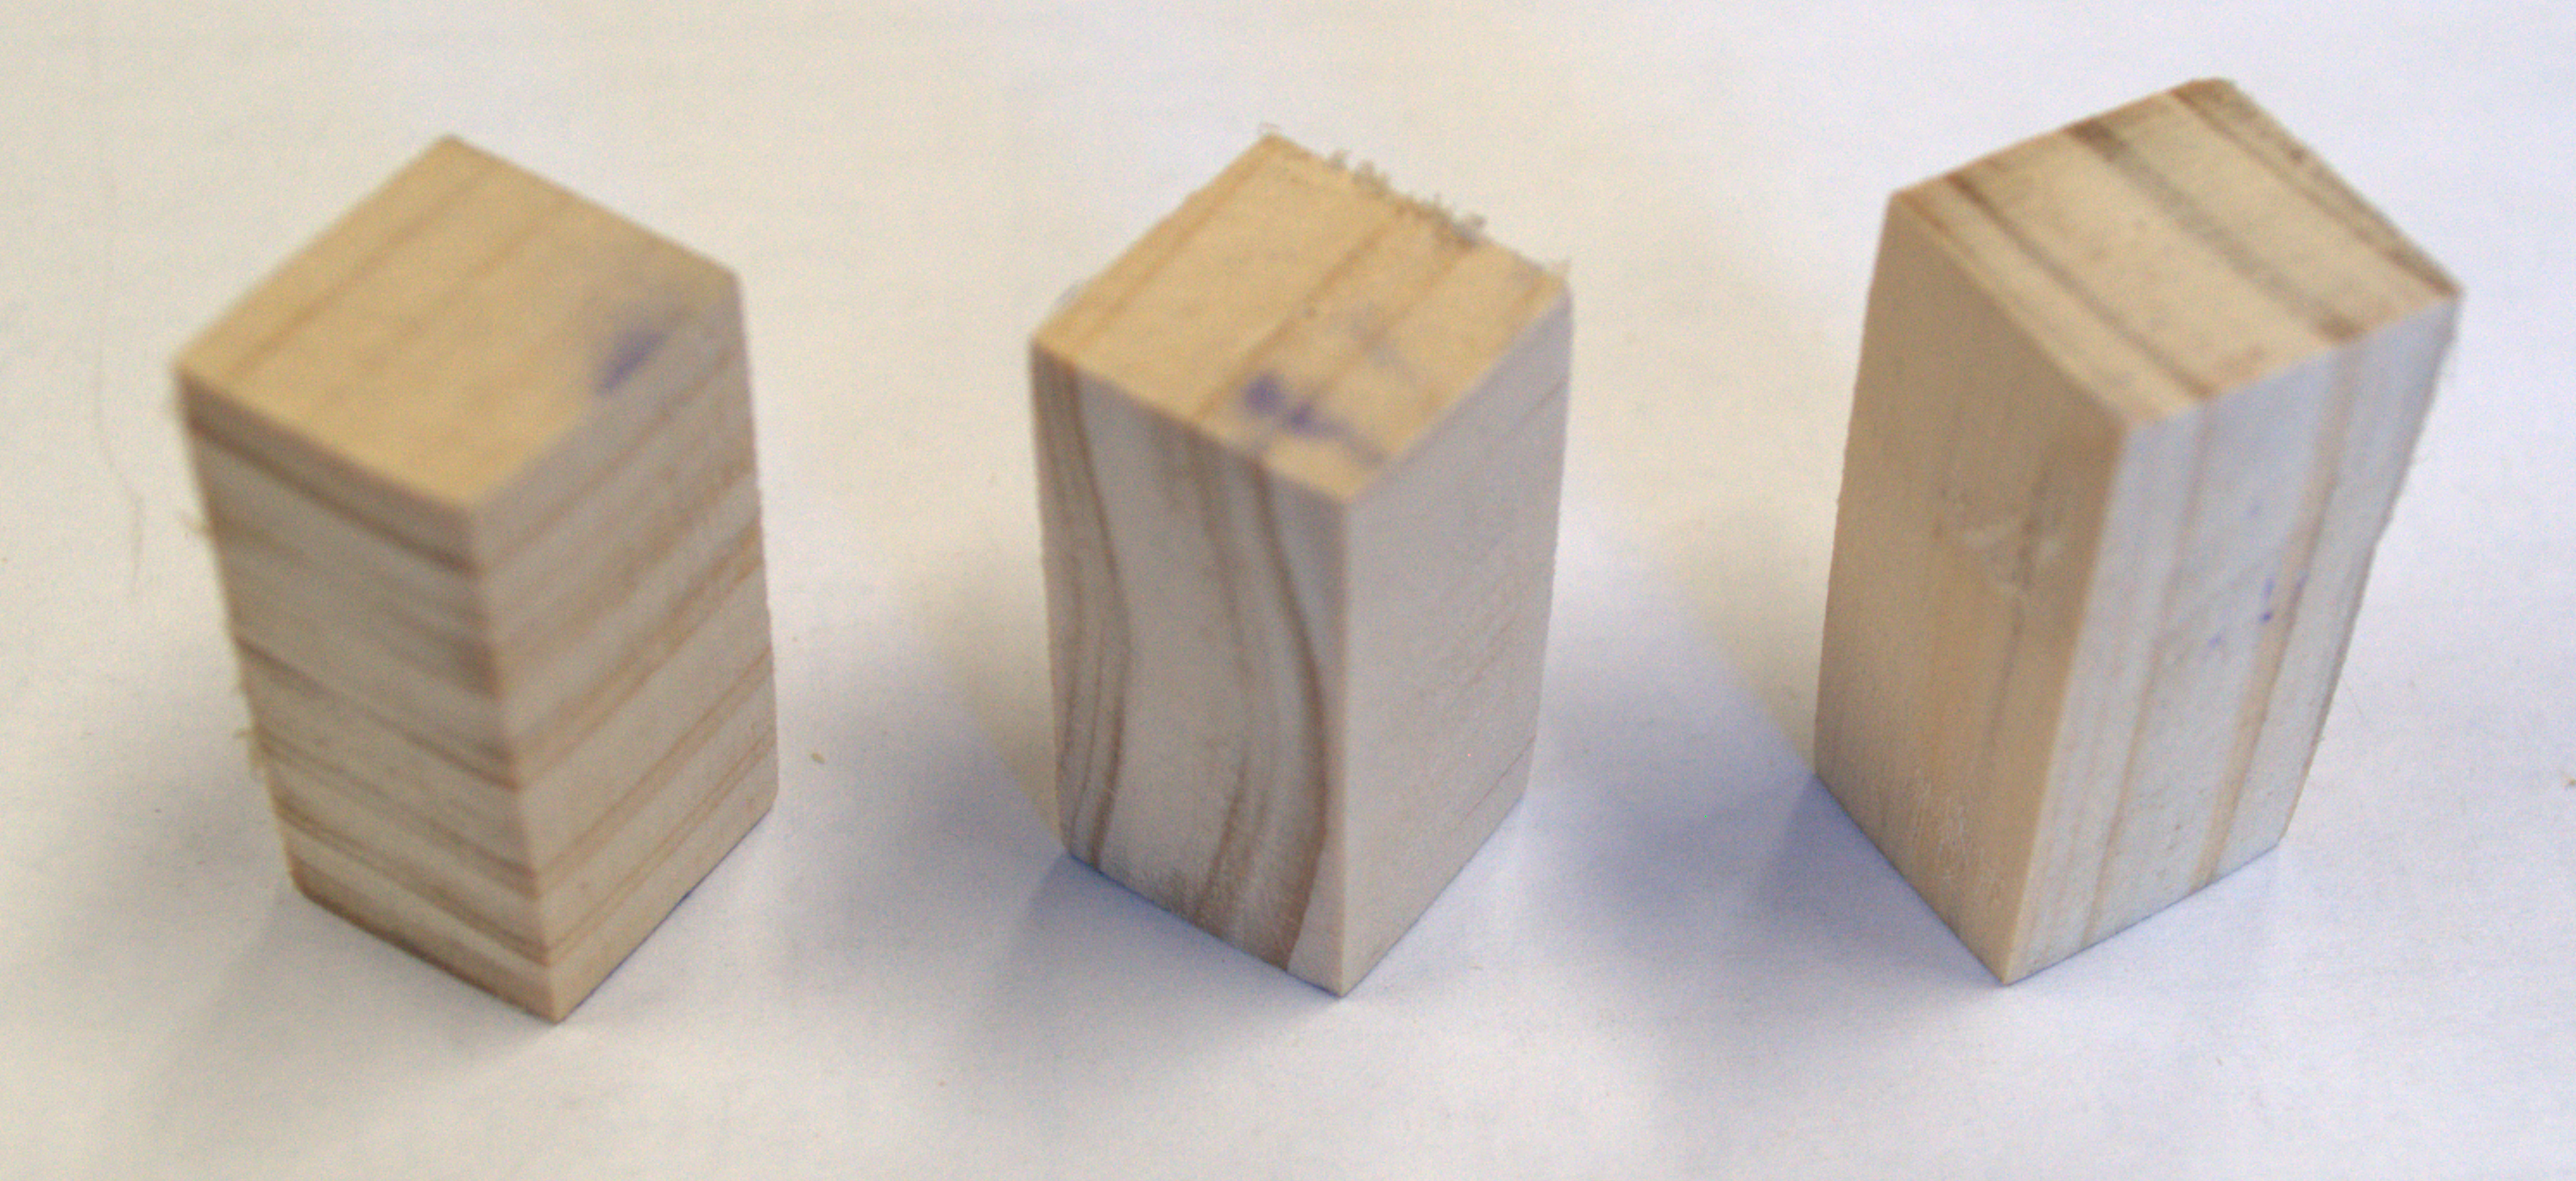
\includegraphics[width=0.7\columnwidth]{figs/compression_samples.png}
% \caption[Compression samples]{\label{fig:compression_samples} Examples of the sample shapes used for compression properties. The samples, labelled in the direction of load applied from left to right are \(r\), \(t\) and \(l\). The vertical direction is 30 mm with the two other sides being 15 mm each.
% }
% \end{center}
% \end{figure}
%
% \begin{figure}[!ht]
% \begin{center}
% 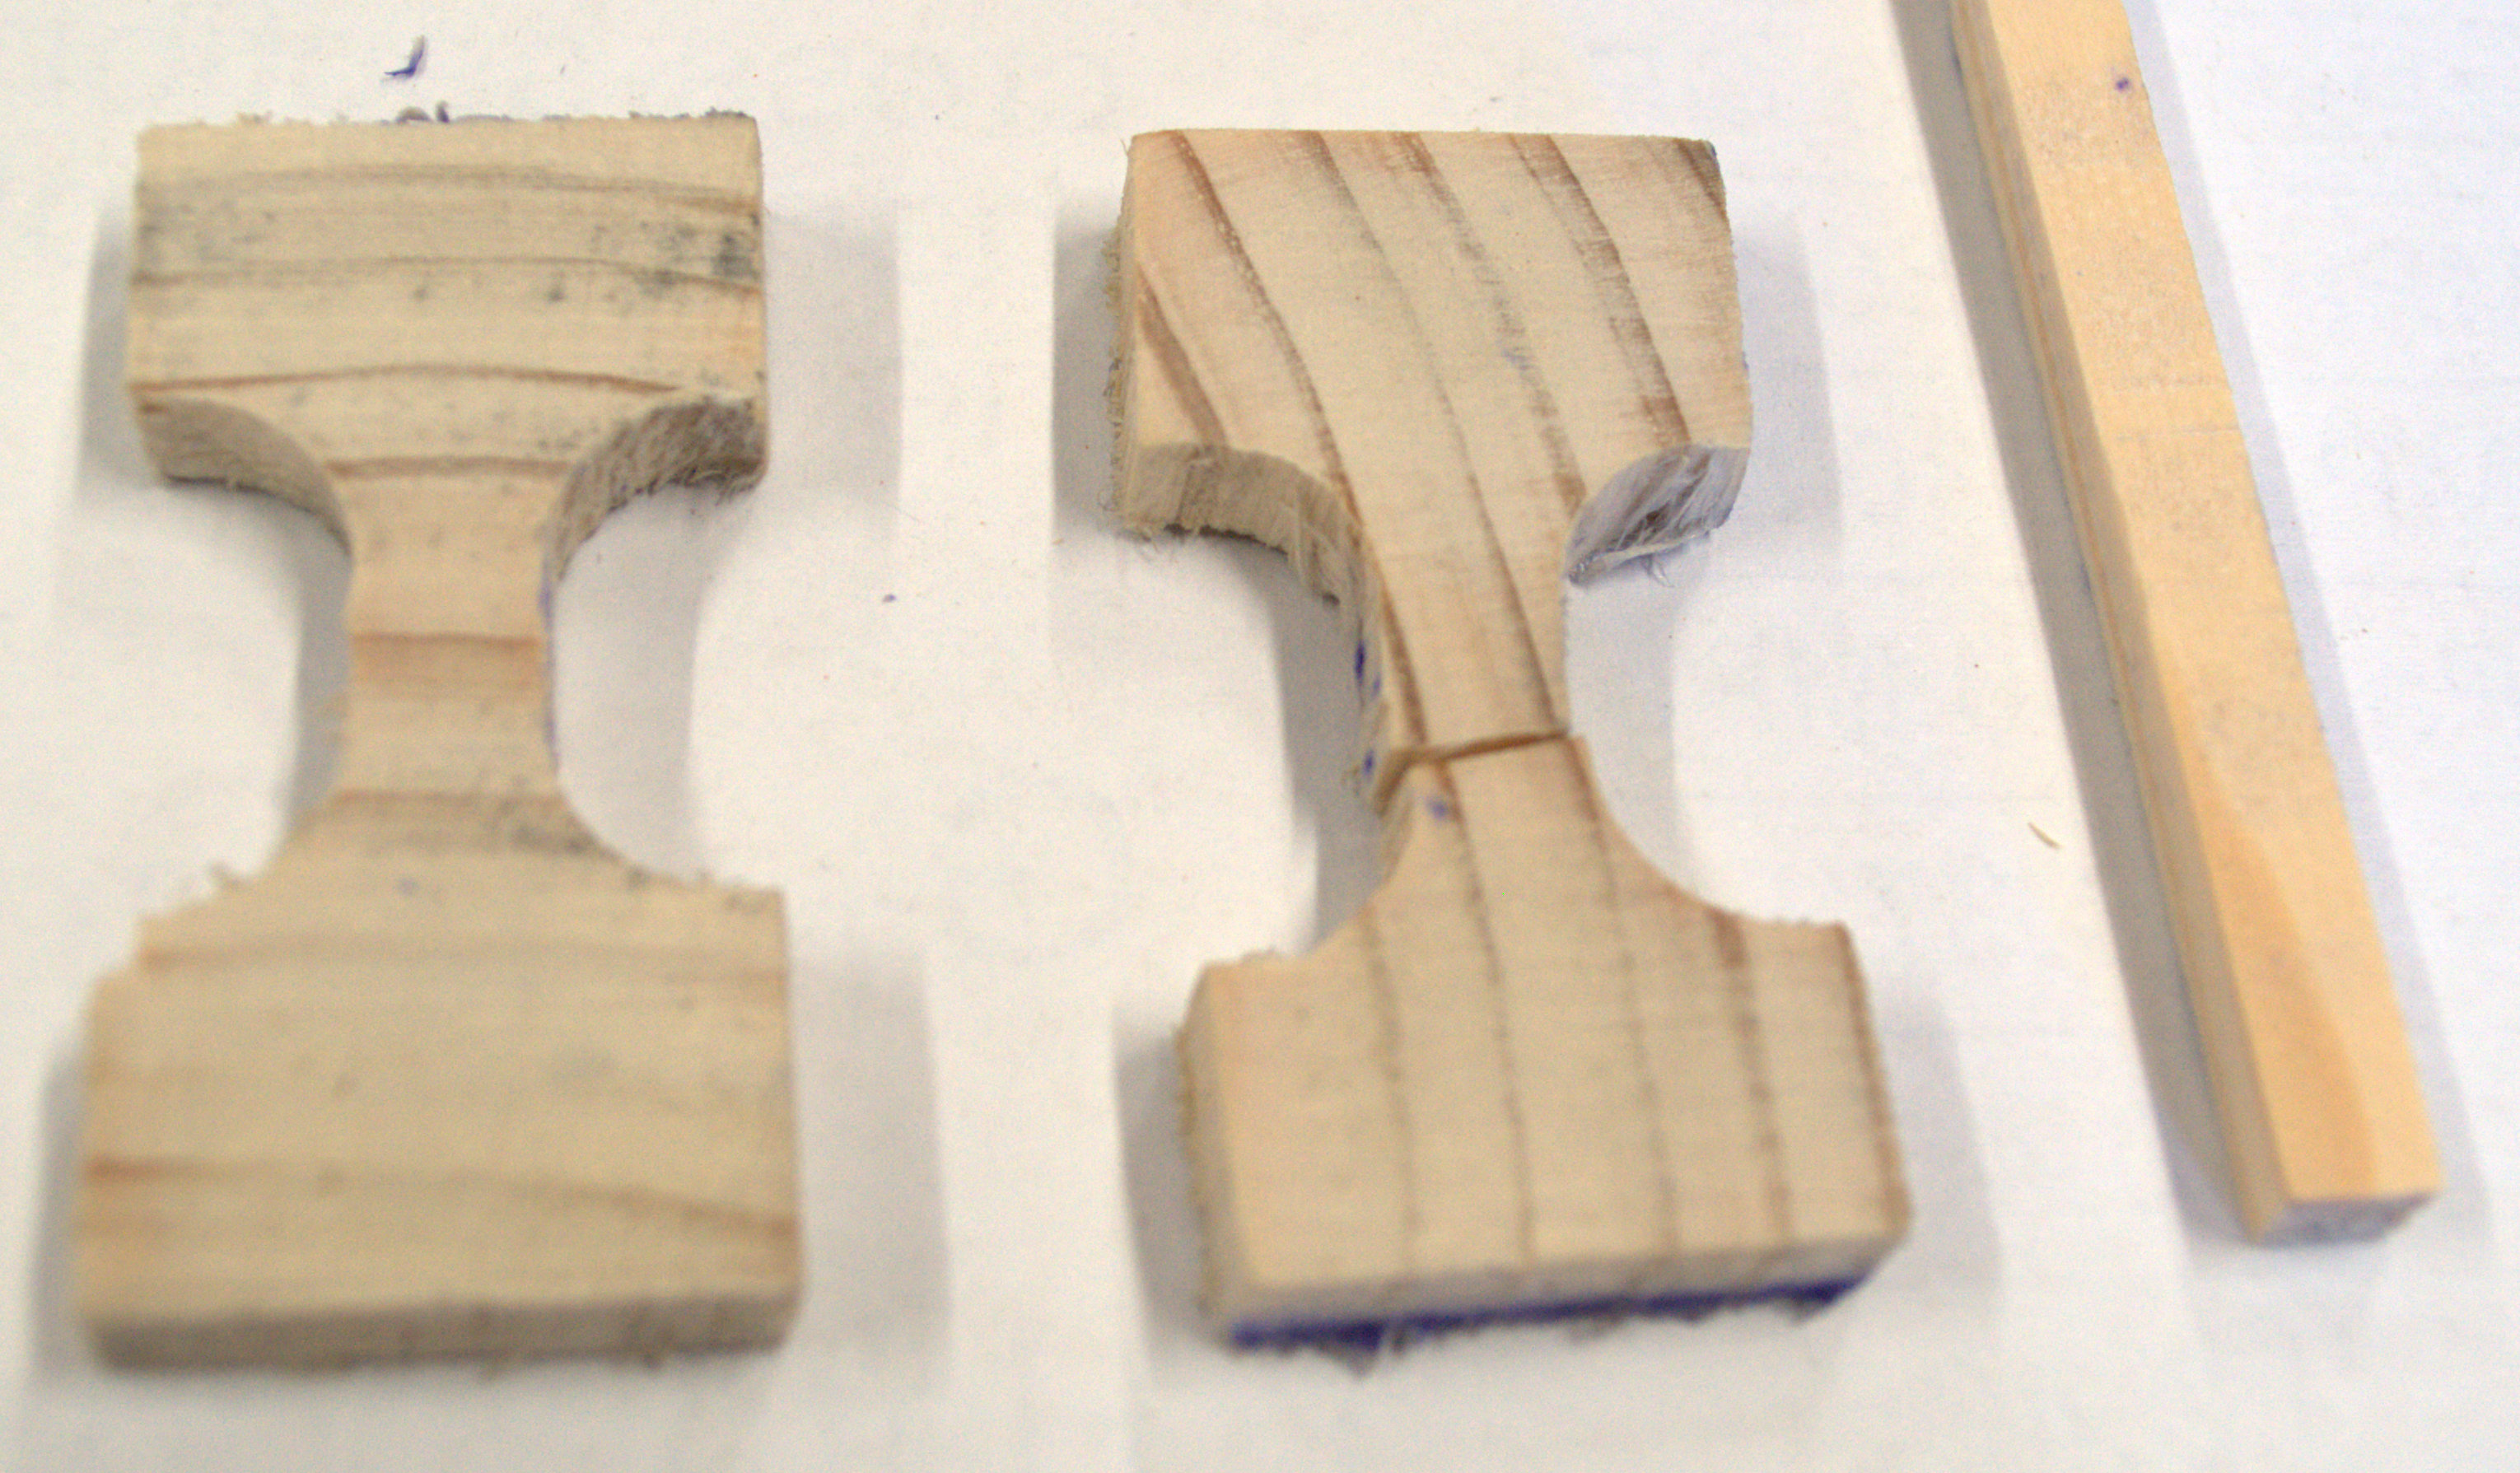
\includegraphics[width=0.7\columnwidth]{figs/tension_samples.png}
% \caption[Tension samples]{\label{fig:tension_samples} Examples of the sample shapes used for tensile property testing. The samples, labelled in the direction of load applied from left to right are \(r\) (radial), \(t\) (tangential) and \(l\) (longitudinal). Samples have a cross sectional area of 6.5 x 6.5 mm at the fracture point. The radial and tangential samples are 100 x 25 x 6.5 mm overall. The longitudinal sample is 200 x 6.5 x 6.5 mm.
% }
% \end{center}
% \end{figure}
%
% \begin{figure}[!ht]
% \begin{center}
% 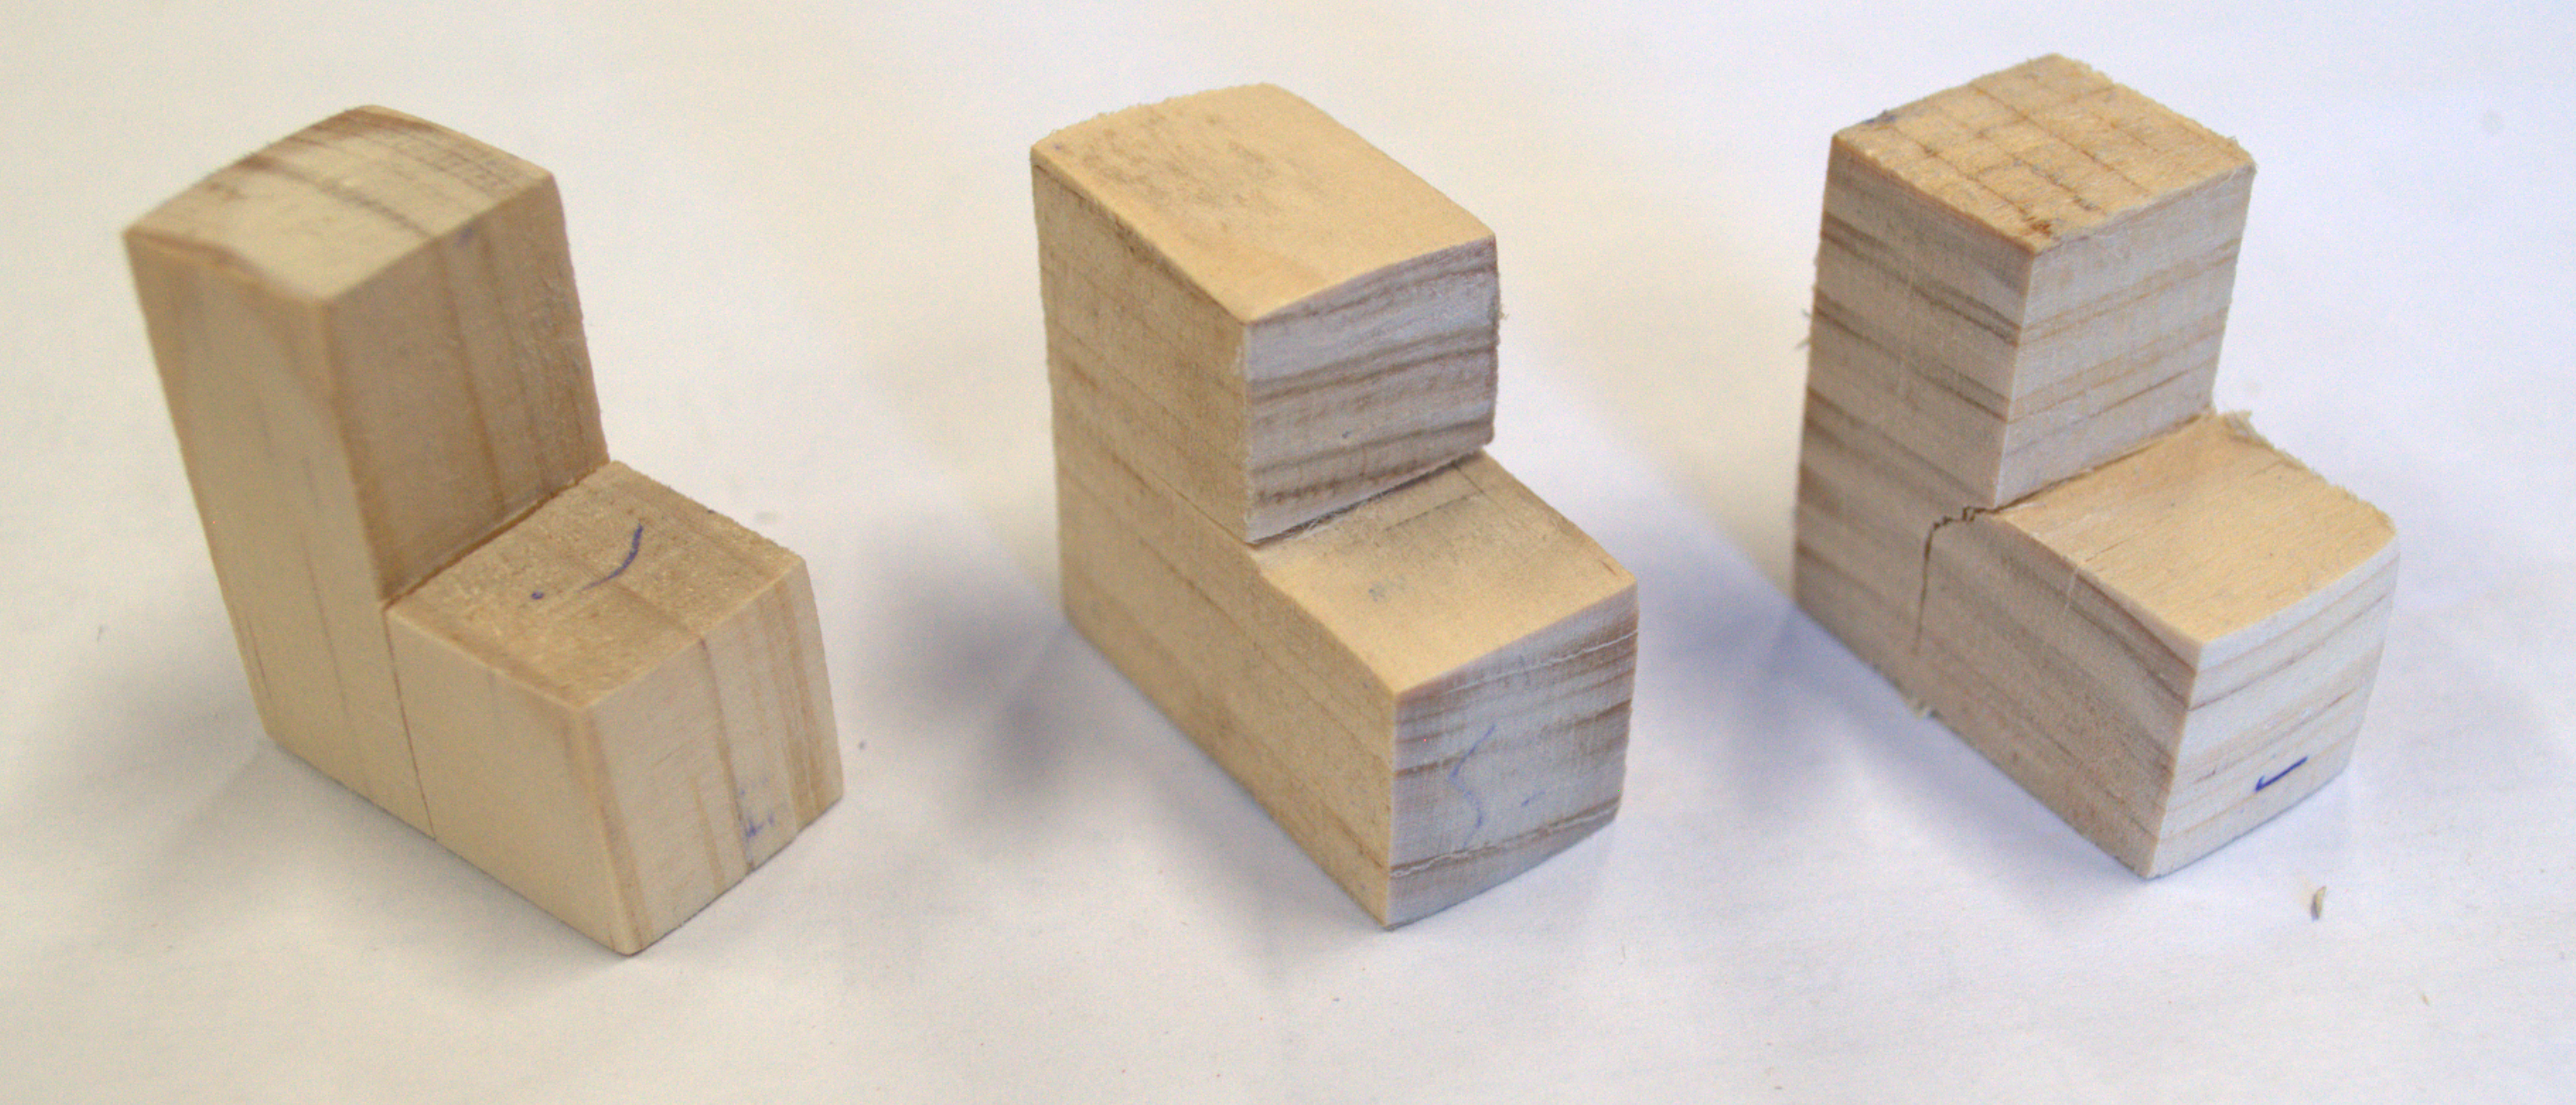
\includegraphics[width=0.7\columnwidth]{figs/shear_samples.jpg}
% \caption[Shear samples]{\label{fig:shear_samples} Examples of the sample shapes used for testing shear properties. The samples, labelled from left to right are the radial tangential plane \(rt\), tangential longitudinal plane \(tl\) and the longitudinal radial plane \(lr\). The samples are 30 mm long by 30 mm high and 15 mm wide, resulting in a 15 x 15 mm shear plane.
% }
% \end{center}
% \end{figure}
%
\begin{figure}[!ht]
\begin{center}
\includegraphics[width=130mm,keepaspectratio]{figs/00_tw_failure.pdf}
\caption[Proportional limit sufaces, no interaction]{\label{fig:yeild, k0} Proportional limit surfaces calculated using \citet{tsai_general_1971} failure criterion with no interaction for all failure planes.
}
\end{center}
\end{figure}
%
% \pagebreak

\begin{table}\label{table:mill samples table}
\caption[Initial properties of samples]{The four samples shown along with their properties known at the time of selection. Green density was measured using a measuring tape to get an approximate volume and field scales to get the weight of the board. Tree tap was used to get the acoustic velocity. Ring number and wood type from visual inspection}
\begin{tabular}{l l l l l}
\hline
Sample & Green Density & Acoustic velocity & Approximate & Type of wood\\
       &               &                   & ring number &              \\
\hline
Stiff Outerwood& high & high & \(>15\) & Sapwood\\
Non-Stiff Outerwood& high & low & \(>15\) & Sapwood\\
Stiff Corewood& low & high & \(<15\) & Heartwood\\
Non-Stiff Corewood& low & low & \(<15\) & Heartwood\\
\hline
\end{tabular}
\end{table}

\begin{table}
\caption[Wood properties]{Table showing the wood properties of the samples. Densities are averages from measuring all of the specimens individually. Disk scanner velocities are averages from individual specimens or a block of no more than six specimens depending on the size and shape. Wood spec velocities are from sections of board  500 mm in length, which were not used for specimens, taken in wet condition. MFA is obtained from x-ray diffraction after testing and drying. }
\label{table:init properties}
\begin{tabular}{l l l l l}
\hline
Property & Stiff Outerwood & Non-Stiff Outerwood & Stiff Corewood & Non-Stiff
Corewood\\
\hline
Green Density, \(kg/m^3\) & 1143 (3) & 1099 (9) & 933 (21) & 818 (22) \\
%Standard Error, \(kg/m^3\) & 3 & 9 & 21 & 22 \\
Dry Density,  \(kg/m^3\) & 531 (5)& 458 (9) & 438 (8) & 393 (5)\\
%Standard Error,  \(kg/m^3\) & 5 & 9 & 8 & 5 \\
Acoustic Velocity \(m/s\) & 4651 (8) & 4221 (26)& 4191 (34)& 3413 (14)\\
Disk Scanner (green)      &          &          &          &           \\
%Standard Error, \(m/s\) & 8 & 26 & 34 & 14\\
Acoustic Velocity  \(m/s\) & 3490 & 3470 & 3470 & 2700\\
Wood Spec (green)          &      &      &      &      \\
Wood Type & outerwood & outerwood & corewood? & corewood \\
Ring Number & \(>15\) & \(>15\)&\(<15\) & \(<15\)  \\
MFA, \(Degrees\) & 7 & 8 & 9 & 21  \\
Standard Deviation & 9 & 12 & 11 & 12 \\
of MFA \(Degrees\)&   &  &   &   \\
\hline
\end{tabular}
\end{table}

\begin{table}
\caption[Experimental Youngs Moduli]{Young's Moduli obtained from various UTM tests. The first letter is the direction of force, the second, the face which was recorded and the third \(t\) is a tension force and \(c\) is a compressive force. Capital letters indicate the shear moduli in the given plane. }
\label{table:youngs moduli}
\begin{tabular}{lllllllll}
\hline
Direction& Stiff Outerwood && Non-Stiff Outerwood && Stiff Corewood && Non-Stiff Corewood &\\
 & \(E\)&\(SE\)& \(E\)&\(SE\)& \(E\)&\(SE\)& \(E\)&\(SE\)\\
\hline
\(rt_t\) in \(GPa\) & 0.40 & 0.11 & 0.24 & 0.05 & 0.13 & 0.01 & 0.16 & 0.01 \\
\(rt_c\) in \(GPa\) & 0.58 & 0.08 & 0.36 & 0.10 & 0.39 & 0.03 & 0.47 & 0.13 \\
\(rl_t\) in \(GPa\) & 0.62 & 0.10 & 0.13 & 0.04 & 0.37 & 0.11 & 0.12 & 0.02 \\
\(rl_c\) in \(GPa\) & 0.57 & 0.07 & 0.58 & 0.09 & 0.45 & 0.07 & 0.54 & 0.10 \\
\(tr_t\) in \(GPa\) & 0.13 & 0.01 & 0.22 & 0.04 & 0.20 & 0.02 & 0.09 & 0.01 \\
\(tr_c\) in \(GPa\) & 0.33 & 0.03 & 0.35 & 0.07 & 0.29 & 0.07 & 0.26 & 0.02 \\
\(tl_t\) in \(GPa\) & 0.30 & 0.11 & 0.08 & 0.01 & 0.14 & 0.01 & 0.14 & 0.02 \\
\(tl_c\) in \(GPa\) & 0.37 & 0.04 & 0.36 & 0.03 & 0.22 & 0.02 & 0.29 & 0.05 \\
\(lr_t\) in \(GPa\) & 10.74 & 1.83 & 3.78 & 0.93 & 3.03 & 0.90 & 4.33 & 1.51 \\
\(lr_c\) in \(GPa\) & 3.10 & 0.11 & 1.02 & 0.50 & 3.76 & 0.80 & 4.04 & 0.61 \\
\(lt_t\) in \(GPa\) & 11.74 & 2.18 & 4.69 & 1.13 & 3.23& 1.50 & 4.05 & 1.17 \\
\(lt_c\) in \(GPa\) & 7.47 & 1.60 & 1.74 & 0.61 & 4.65 & 1.06 & 5.85 & 1.18 \\
\(TL\) in \(MPa\)   & 111.7 & 7.3 & 211.1& 3.9  & 107.0& 1.2  & 125.8& 5.4 \\
\(LR\) in \(MPa\)   & 59.7 & 1.9  & 34.4 & 1.2  & 38.5 & 1.7  & 29.5 & 1.1 \\
\(RT\) in \(MPa\)   & 45.9 & 1.3  & 22.8 & 1.7  & 22.5 & 1.4  & 39.0 & 0.8 \\
\hline
\end{tabular}
\end{table}


\begin{table}
\caption[Poisson ratios]{\(v\) is the Poisson ratio and \(SE\) is the standard error on the ratio. First letter is the direction of force, the second the face which was recorded and the third \(t\) is a tension force and \(c\) is a compressive force.}
\label{table:poisson ratios}
\begin{tabular}{lllllllll}
\hline
Direction& Stiff Outerwood&& Non-Stiff Outerwood&& Stiff Corewood&&Non-Stiff Corewood&\\
 & \(v\)&\(SE\)& \(v\)&\(SE\)& \(v\)&\(SE\)& \(v\)&\(SE\)\\
\hline
\(rt_t\) & 0.21 & 0.10 & 0.30 & 0.08& 0.27 & 0.12& 0.08 & 0.01\\
\(rt_c\) & 0.64 & 0.04 & 0.52 & 0.09& 0.60 & 0.05& 0.49 & 0.17\\
\(rl_t\) & 0.26 & 0.08& 0.04 & 0.02& 0.31 & 0.15& 0.15 & 0.06 \\
\(rl_c\) & 0.14 & 0.04& 0.15 & 0.05& 0.22 & 0.14& 0.17 & 0.13 \\
\(tr_t\) & 0.20 & 0.03 & 0.19 & 0.05& 0.53 & 0.22& 0.02 & 0.01\\
\(tr_c\) & 0.47 & 0.10 & 0.33 & 0.04& 0.39 & 0.08& 0.42 & 0.05\\
\(tl_t\) & 0.15 & 0.05 & 0.09 & 0.03& 0.04 & 0.02& 0.62 & 0.08\\
\(tl_c\) & 0.10 & 0.02 & 0.08 & 0.04& 0.18 & 0.08& 0.08 & 0.03\\
\(lr_t\) & 0.24 & 0.08& 0.42& 0.18& 0.30 & 0.01& 0.35 & 0.14 \\
\(lr_c\) & 0.26 & 0.05& 0.41 & 0.13& 0.36 & 0.08& 0.44 & 0.09 \\
\(lt_t\) & 0.48 & 0.14& 0.29 & 0.10& 0.39 & 0.17& 0.21 & 0.05 \\
\(lt_c\) & 0.41 & 0.08& 0.16 & 0.06& 0.37 & 0.09& 0.42 & 0.14 \\
\hline
\end{tabular}
\end{table}

% \begin{table}
% \caption[Orthotropic material constants]{Optimized values for the orthotropic assumption. All Poisson ratios used are from compression tests for reasons described in section \ref{sec:orthotropic_assumption} the moduli are reported from both the compression and tension tests}
% \label{table:optermised vals}
% \begin{tabular}{l l l l l l l l l l}
% \hline
% Compression	&	&	&	&	&	&	&	&	&\\
% Axial direction	&Long-rad	&	&	&	&	&Long-tan	&	&	&\\
% Constant	&Stiff Outerwood	&Non-Stiff Outerwood	&Stiff Corewood	&Non-Stiff Corewood	&	&Stiff Outerwood	&Non-Stiff Outerwood	&Stiff Corewood	&Non-Stiff Corewood\\
% \(E_r\)	&0.58	&0.39	&0.43	&0.29	&	&0.66	&0.49	&0.39	&0.29\\
% \(E_t\)	&0.33	&0.35	&0.29	&0.26	&	&0.37	&0.35	&0.29	&0.26\\
% \(E_l\)	&3.10	&1.04	&4.17	&4.04	&	&4.33	&1.45	&4.63	&3.56\\
% \(v_{rt}\)	&0.64	&0.36	&0.60	&0.49	&	&0.64	&0.46	&0.60	&0.49\\
% \(v_{rl}\)	&0.06	&0.15	&0.04	&0.03	&	&0.06	&0.15	&0.03	&0.04\\
% \(v_{tr}\)	&0.37	&0.33	&0.41	&0.42	&	&0.36	&0.33	&0.45	&0.42\\
% \(v_{tl}\)	&0.05	&0.05	&0.03	&0.04	&	&0.05	&0.04	&0.03	&0.04\\
% \(v_{lr}\)	&0.30	&0.41	&0.36	&0.44	&	&0.36	&0.45	&0.36	&0.44\\
% \(v_{lt}\)	&0.45	&0.16	&0.37	&0.57	&	&0.56	&0.16	&0.41	&0.50\\
% &	&	&	&	&	&	&	&	&\\
% \hline
% &	&	&	&	&	&	&	&	&\\
% Tension	&	&	&	&	&	&	&	&	&\\
% Axial direction	&Long-rad	&	&	&	&	&Long-tan	&	&	&\\
% Constant	&Stiff Outerwood	&Non-Stiff Outerwood	&Stiff Corewood	&Non-Stiff Corewood	&	&Stiff Outerwood	&Non-Stiff Outerwood	&Stiff Corewood	&Non-Stiff Corewood\\
% \(E_r\)&0.40	&0.34	&0.14	&0.16	&	&0.22	&0.34	&0.14	&0.16\\
% \(E_t\)&0.16	&0.22	&0.16	&0.09	&	&0.16	&0.23	&0.16	&0.09\\
% \(E_l\)	&5.06	&3.73	&2.26	&1.37	&	&4.98	&2.76	&2.26	&1.76\\
% \(v_{rt}\)&0.64	&0.52	&0.50	&0.75	&	&0.64	&0.52	&0.50	&0.73\\
% \(v_{rl}\)&0.02	&0.05	&0.02	&0.05	&	&0.01	&0.05	&0.02	&0.04\\
% \(v_{tr}\)&0.26	&0.33	&0.56	&0.42	&	&0.47	&0.34	&0.56	&0.42\\
% \(v_{tl}\)	&0.02	&0.01	&0.03	&0.04	&	&0.02	&0.01	&0.03	&0.04\\
% \(v_{lr}\)	&0.26	&0.55	&0.36	&0.44	&	&0.26	&0.41	&0.36	&0.44\\
% \(v_{lt}\)	&0.64	&0.16	&0.37	&0.55	&	&0.64	&0.16	&0.37	&0.69\\
%
% \hline
% \end{tabular}
% \end{table}

\begin{table}
\caption[Averaged orthotropic material constants]{Optimized values for the orthotropic assumption. All Poisson ratios used are from compression teststhe moduli are reported calculated from averages of tension and compression. In the \(r\) and \(t\) directions this is the average of tension and compression from the camera viewing the \(rt\) or \(tr\) plane. In the longitudinal direction it is the average of all four image sets.}
\label{table:optermised vals average}
\begin{tabular}{lllll}
\hline
Average	&	    &	    &	    &   \\
Direction&  	&	    &	    &   \\
	    &Stiff Outerwood	    &Non-Stiff Outerwood	    &Stiff Corewood	    &Non-Stiff Corewood \\
\(E_r\)	    &0.49	&0.30	&0.26	&0.31\\
\(E_t\)	    &0.25	&0.19	&0.24	&0.17\\
\(E_l\)	    &4.36	&2.81	&3.50	&2.38\\
\(v_{rt}\)	&0.64	&0.54	&0.60	&0.77\\
\(v_{rl}\)	&0.03	&0.05	&0.03	&0.06\\
\(v_{tr}\)	&0.33	&0.33	&0.55	&0.42\\
\(v_{tl}\)	&0.03	&0.01	&0.03	&0.04\\
\(v_{lr}\)	&0.29	&0.47	&0.36	&0.44\\
\(v_{lt}\)	&0.60	&0.16	&0.37	&0.50\\

\hline
\end{tabular}
\end{table}


\begin{table}
\caption[Proportional limits]{Proportional limit values in \(MPa\) the first letter is the direction of force, the second the face which was recorded and the third \(t\) is a tension force and \(c\) is a compressive force. Capital letters are the planes of shear.}
\label{table:yield points}
\begin{tabular}{lllllllll}
\hline
Direction & Stiff Outerwood && Non-Stiff Outerwood && Stiff Corewood && Non-Stiff Corewood & \\
 & \(S\)&\(SE\)& \(S\)&\(SE\)& \(S\)&\(SE\)& \(S\)&\(SE\)\\
\hline
\(rt_t\) & 0.8 & 0.2& 1.3& 0.5& 1.2 & 0.3& 0.9 & 0.1 \\
\(rt_c\) & -3.2 & 0.1& -2.5& 0.2& -2.1 & 0.1& -3.2 & 0.3 \\
\(rl_t\) & 1.0 & 0.1& 0.8& 0.2& 1.7 & 0.4& 0.5 & 0.1 \\
\(rl_c\) & -3.3 & 0.2& -2.6& 0.1&-2.3 & 0.1& -3.3 & 0.2 \\
\(tr_t\) & 0.8 & 0.2& 0.7& 0.2& 0.9 & 0.1& 0.6 & 0.1 \\
\(tr_c\) & -2.7 & 0.1& -2.4& 0.3& -1.8 & 0.2& -2.0 & 0.2 \\
\(tl_t\) & 1.0 & 0.3& 0.5& 0.1& 0.8 & 0.2& 0.8 & 0.2 \\
\(tl_c\) & -2.6 & 0.2& -2.8& 0.2& -2.0 & 0.1& -2.3 & 0.3 \\
\(lr_t\) & 46.0 & 7.5& 26.0& 1.3& 7.6 & 1.8& 21.8 & 4.1 \\
\(lr_c\) & -17.4 & 1.0& -6.6& 2.9& -14.0 & 1.1& -17.6 & 1.9 \\
\(lt_t\) & 35.3 & 3.8& 27.0& 4.5& 9.6 & 2.4& 20.6 & 2.4 \\
\(lt_c\) & -15.5 & 1.5& -8.5& 3.5& -13.6 & 1.6& -21.4 & 2.8 \\
\(TL\) & 2.2 & 0.4& 4.5& 0.3& 2.7 & 0.2&3.2 & 0.3 \\
\(LR\) & 1.8 & 0.1& 0.9& 0.2& 1.6 & 0.3& 1.3 & 0.1 \\
\(RT\) & 1.1 & 0.2& 0.6& 0.2& 0.7 & 0.1& 0.9 & 0.1 \\
\hline
\end{tabular}
\end{table}

\begin{table}
\caption[Ultimate strength]{Ultimate strength reported in \(MPa\). Only tensile strength is reported, the first letter is the direction of the force, second is the plane of imaging.}
\label{table:ultimate strength}
\begin{tabular}{lllllllll}
\hline
Direction& Stiff Outerwood && Non-Stiff Outerwood && Stiff Corewood && Non-Stiff Corewood &\\
 & \(S\)&\(SE\)& \(S\)&\(SE\)& \(S\)&\(SE\)& \(S\)&\(SE\)\\
\hline
\(rt\) & 3.1 & 0.3& 3.1& 0.3& 2.9 & 0.2& 2.2 & 0.2 \\
\(rl\) & 3.1 & 0.3& 3.0& 0.3& 2.8 & 0.3& 2.2 & 0.2 \\
\(tr\) & 2.1 & 0.4& 1.6& 0.3& 1.9 & 0.1& 2.1 & 0.2 \\
\(tl\) & 2.1 & 0.5& 1.4& 0.3& 1.9 & 0.1& 2.1 & 0.2 \\
\(lr\) & 64.2 & 5.9& 45.2& 4.6& 21.2 & 1.6& 32.6 & 2.9 \\
\(lt\) & 65.0 & 5.7& 43.6& 5.1& 20.0 & 1.9& 32.8 & 2.9 \\
\hline
\end{tabular}
\end{table}

\begin{landscape}
\begin{table}
\scriptsize
\caption[Comparison with values from the literature]{Comparison of literature values with the findings in this study. Values are aproximate as a number of them were taken from published plots. All Moduli in \(GPa\).}
\label{table:lit_comp}
\begin{tabular}{lllllllllllllll}
\hline
Reference & Test & Species& \(E_r\) & \(E_t\) & \(E_l\) & \(G_{tl}\) & \(G_{lr}\) & \(G_{rt}\) & \(v_{rt}\) &\(v_{rl}\)  & \(v_{tr}\)   & \(v_{tl}\)&\(v_{lr}\)&\(v_{lt}\)\\
\hline
This work & Static & \textit{Pinus radiata}& 0.26  & 0.17 & 2.38 & 0.11 & 0.03 & 0.02 & 0.54 & 0.03 & 0.33 & 0.01 & 0.29 &0.16\\
(Range)& && 0.49 & 0.25 & 4.36 & 0.21 & 0.06 & 0.05 &  0.77 & 0.06 & 0.55 & 0.04 & 0.47 & 0.60\\
\cite{ozyhar_moisture-dependent_2013}& Static & \textit{Fagus sylvatica} &1.14  & 0.53 & 9.14 &  &  &  & 0.19  & 0.39 & 0.47 & 0.5 & 0.04 & 0.03\\
(Range)&  &  &2.33  & 1.05 & 14.54 &  &  &  & 0.41  & 0.55 & 0.76 & 0.87 & 0.2 & 0.11\\
\cite{henrik_three_2013}& &  & 0.8 & 0.5 & 12 & 0.7 & 0.7 & 0.05 &   & 0.02 & 0.3 & 0.02 && \\
\cite{raffaele_morphology_2011}& Hybrid &\textit{Picea Abies} & 0.236 & 0.387 & 10.4 & 0.65 & 0.597 & 0.029 & 0.42  & 0.018 &  &0.017  &  & \\
\cite{mackenzie-helnwein_rate-independent_2005}& Hybrid & Spruce & 0.7 & 0.5 & 13 & 0.47 & 0.63 & 0.22 & 0.38  &  &  & 0.013 & 0.5 & \\
\cite{ormarsson_moisture-related_2005}& Hybrid & \textit{Pinus radiata} & 0.7 & 0.2 & 5 & 0.6 & 1 & 0.05 &   &  &  &  &  & \\
(Range)&   & & 2.2 & 0.7 & 19 & 1.2 & 2 & 0.15 &   &  &  &  &  & \\
\cite{qing_3d_2009}& Theoretical& &  & 2.202 & 20.25 & 1.94 &  & 1.4 &   &  &  &  &  & \\
\cite{harrington_hierarchical_2002}& Theoretical & \textit{Pinus radiata} & 0.56 & 0.23 & 5.61 & 1.0 & 1.20 & 0.08 &   & 0.42 & 0.38 & 0.37 &  & \\
(Range)&& &3.08 & 3.08 & 9.33 & 2.18 & 2.07 & 0.79 &  & 0.48  & 1.23 & 0.45 &  &   \\
\cite{persson_micromechanical_2000}& Theoretical& Spruce &0.67  & 0.08 & 7.7 & 0.40 &0.68  & 0.009 &   & 0.009 & 0.124 & 0.006 &  & \\
(Range)& & & 1.57 & 2.1 &36.4 &1.77  & 1.76 & 0.043 &   & 0.057 & 0.241 & 0.054 &  & \\
\hline
\end{tabular}
\end{table}
\end{landscape}

\begin{table}
\caption[Further literature comparison]{Literature values for the longitudinal elastic moduli. Values are aproximate as a number of them were taken from published plots. All moduli in \(GPa\).}
\label{table:lit_comp_long}
\begin{tabular}{llll}
\hline
Reference & Test & Species & \(E_l\) \\
\hline
\cite{watt_modelling_2006}&Dynamic &\textit{Pinus radiata} &  2 - 7 \\
\cite{waghorn_influence_2007}&Dynamic  &  & 5 - 9 \\
\cite{lindstrom_stiffness_2004}&Dynamic  &   & 2 - 4.8 \\
\cite{xinguo_transcriptome_2011}&Dynamic  &  & 3 - 6 \\
\cite{s_modelling_2008}&Dynamic  & &  2.4 - 5.9 \\
\cite{lasserre_influence_2009}&Dynamic & &  2.7 - 4.2 \\
\cite{watt_influence_2011}& Silviscan &  & 3 - 15\\
\cite{downes_relationship_2002}&Silviscan & &   11.5 - 13.5 \\
\cite{watt_determining_2010}&Silviscan &  &  1.4 - 21.6\\
\cite{s_development_2010}&Silviscan & &   3 - 18\\
\cite{xu_effects_2004}& Static & &  4.8 - 14.9\\
\cite{lindstrom_methods_2002}& Static & & 2.5 - 6 \\
\hline
\end{tabular}
\end{table}

\end{document}





